\documentclass[tikz,border=1mm]{standalone}
\usetikzlibrary{matrix,chains,positioning,decorations.pathreplacing,arrows,shapes.geometric}

% Code modified from here https://tex.stackexchange.com/questions/505741/architecture-neural-network-with-weights

\begin{document}
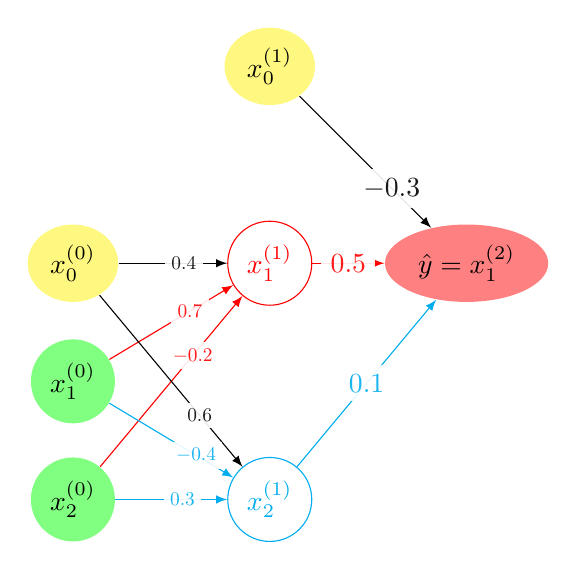
\begin{tikzpicture}[>=latex]

% Step 1 
\path
(0,0)     node[circle,draw,red, align=center] (S1) {$x^{(1)}_1$} 
+(-2.5,0) node[ellipse,fill=yellow!50]  (b) {$x^{(0)}_0$}
+(-2.5,-1.5)  node[circle,fill=green!50]  (x1) {$x^{(0)}_1$}
+(-2.5,-3)    node[circle,fill=green!50]  (x2) {$x^{(0)}_2$}
;

\draw[->, black] (b)--(S1) node[pos=.6, fill=white, opacity=.9, scale=0.7]{$0.4$};
\draw[->, red] (x1)--(S1) node[pos=.65,fill=white, opacity=.9, scale=0.7]{$0.7$};
\draw[->, red] (x2)--(S1) node[pos=.65,fill=white, opacity=.9, scale=0.7]{$-0.2$}; 
% End step 1 

% Step 2 
\path 
(0,-3)     node[circle,draw,cyan, align=center] (S2) {$x^{(1)}_2$};
\draw[->, black] (b)--(S2) node[pos=.7,fill=white, opacity=.9, scale=0.7]{$0.6$};
\draw[->, cyan] (x1)--(S2) node[pos=.7,fill=white, opacity=.9, scale=0.7]{$-0.4$};
\draw[->, cyan] (x2)--(S2) node[pos=.6,fill=white, opacity=.9, scale=0.7]{$0.3$}; 
% end of Step 2

% % % step 3: 
\path 
(0,2.5)  node[ellipse,fill=yellow!50, align=center]  (hidden_bias) {$x^{(1)}_0$}  % bias neuron for hidden 
(2.5,0)  node[ellipse,fill=red!50, align=center]  (y) {$\hat{y}=x^{(2)}_1$}; % final output neuron

\draw[->, black] (hidden_bias)--(y) node[pos=.7, fill=white, opacity=.9]{$-0.3$};
% \draw [black, ->] (hidden_bias) to [out=0,in=90] (y) node[above=12mm, fill=white, opacity=.9]{$v_{0}$};
\draw[->, red] (S1)--(y) node[pos=.5,fill=white, opacity=.9]{$0.5$};
\draw[->, cyan] (S2)--(y) node[pos=.5,fill=white, opacity=.9]{$0.1$};

\end{tikzpicture}
\end{document}
